\subsection{Analyse der Eventlogs}
Zur Analyse der Eventlogs wurde das Programm Disco von Fluxicon verwendet \cite{ProcessMiningAutomated}. Es erlaubt das automatische Erstellen von verschiedenen Prozess-Modellen, welche direkt aus den Rohdaten generiert werden. Die Grafik \ref{fig:Prozessmodell} zeigt das zu den Eventlogs generierte Prozessmodell. Aktivitäten werden hier durch blau eingefärbte Rechtecke dargestellt. Es ist leicht zu erkennen, dass die Anzahl der Aufkommen der einzelnen Aktivitäten sich in der stärke des Blautons wieder spiegelt. Das $\bigtriangledown$ Symbol signalisiert den Startpunkt alles Prozessdurchläufe. Ein Prozessdurchlauf wäre hier beispielsweise IQR: an Outlier $\rightarrow$ LOF: an Outlier $\rightarrow$ Iforest: Maybe Outlier $\rightarrow$ SVM: an Outlier. Diese Prozessdurchläufe lassen sich durch die Pfade zwischen den Aktivitäten erkennen, wobei die dicke der Pfade sich anhand der durchlaufenen Häufigkeiten zeigt. Ein Prozessdurchlauf endet. sobald der Pfad an dem $\square$ Symbol ankommt endet dieser. 
\begin{figure}[hbt!]
	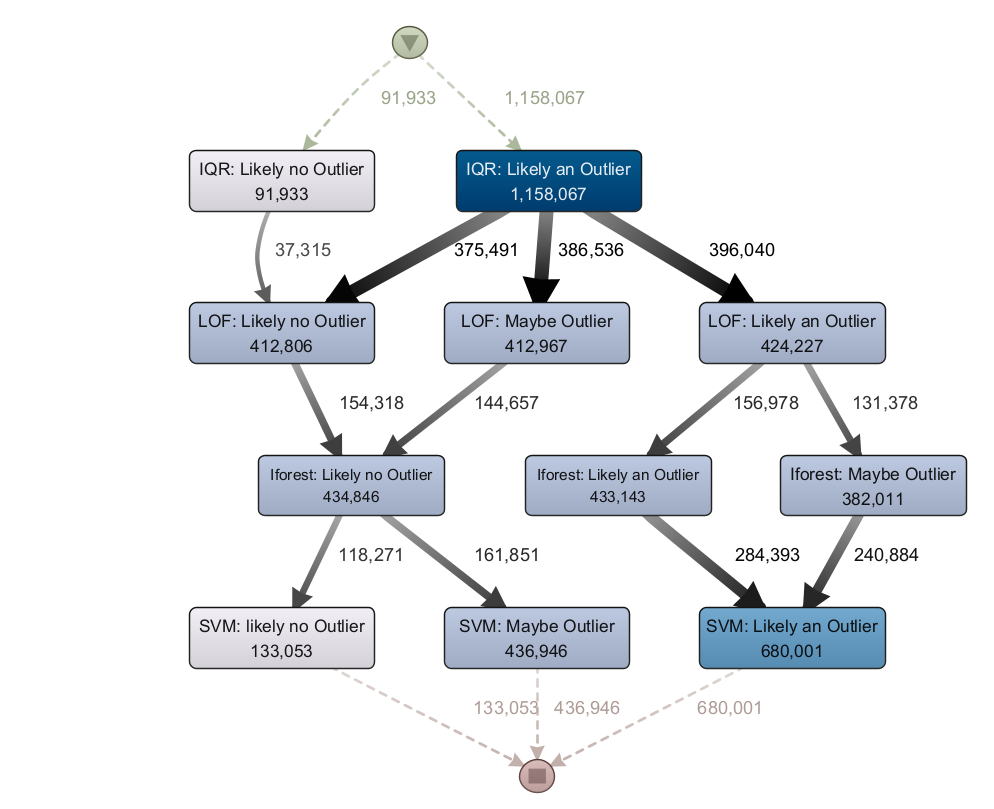
\includegraphics[width=\textwidth]{img/Prozessmodell.png}
	\caption[Prozessmodell]{Prozessmodell}
	\label{fig:Prozessmodell}
\end{figure}
 
\FloatBarrier 

Ein einzelner Prozessdurchlauf lässt sich auch als Case beschreiben. Ein Case spiegelt somit alle Ausprägungen jedes Datenpunkts wieder. Alle Cases, die den selben Ablauf im Prozessmodell haben können durch das Programm in sogenannte Varianten zusammengefasst werden. Eine Variante wäre also zum Beispiel alle Cases, die den Prozessablauf: IQR: an Outlier $\rightarrow$ LOF: Maybe Outlier $\rightarrow$ Iforest: Maybe Outlier $\rightarrow$ SVM: Maybe Outlier $\rightarrow$ an Outlier besitzen. Nachfolgend wurden die verschiedenen Varianten in eigene Gruppen gekapselt. Folgende Gruppen wurden in der Tabelle \ref{tab:gruppierung} erstellt:
\FloatBarrier
\begin{table}[t]
	\centering
	\begin{tabular}{lll}
		\toprule
		\multicolumn{1}{l}{\textbf{Index}} & \textbf{Gruppennummer} & \textbf{Aufteilung} \\ 
		\midrule
		1 & Gruppe 1 & 4 Mal Richtig \\
		2 & Gruppe 2 & 4 Mal Falsch \\
		3 & Gruppe 3 & 3 Mal Richtig, 1 Mal Falsch \\
		4 & Gruppe 4 & 2 Mal Richtig, 2 Mal Falsch \\
		5 & Gruppe 5 & 1 Mal Richtig, 3 Mal Falsch \\
		6 & Gruppe 6 & 3 Mal Richtig, 1 Mal Vielleicht \\
		7 & Gruppe 7 & 2 Mal Richtig, 2 Mal Vielleicht \\
		8 & Gruppe 8 & 1 Mal Richtig, 3 Mal Vielleicht \\
		9 & Gruppe 9 & 3 Mal Falsch, 1 Mal Vielleicht \\
		10 & Gruppe 10 & 2 Mal Falsch, 2 Mal Vielleicht \\
		11 & Gruppe 11 & 1 Mal Falsch, 3 Mal Vielleicht \\
		\bottomrule
	\end{tabular}
	\caption{Gruppierung:}
	\label{tab:gruppierung}
\end{table}
\FloatBarrier

\begin{itemize}
	\item Jetzt Happy Path erklären und aus Gruppe 1 und 2 bilden.
	\item Plot des Happy Paths zeigen und erklären, warum z.b. alle 4 daneben liegen.
	\item Anschließend Plot für alle Gruppen zeigen. Möglicherweise verschiedene Plots für jede Gruppe und innerhalb der Gruppe verschiedene Farben für Outlier und Inlier
	\item Nächste Analyse wäre dann die Gruppen genauer zu betrachten: z.B. Gruppe 7: Welche 2 sind vermehrt richtig und welche 2 sind vermehrt vielleicht
\end{itemize}

\subsection{Analyse der Methoden?}
\subsection{Nutzen von Backpropagationzur Kantengewicht-Bestimmung?}